

\subsection{Sensor Calibration}

A planar checkerboard pattern was used to calibrate all three cameras to obtain both intrinsic and extrinsic parameters.  While the grid pattern is not visible in the depth image, it is nevertheless observed in the reflected IR image whose pixels correspond to the depth pixels.  This enables the use of Zhang's method~\cite{Zhang2000} to calculate the intrinsic parameters including a $2$-parameter radial distortion of each camera.  In this process the poses of all three cameras are also calculated relative to the checkerboard.  The intrinsic and extrinsic parameters are stored as text files, and a Matlab function is provided that reads the parameters and can plot the camera poses as in Fig.~\ref{fig:CameraConfiguration}.


\subsubsection{Noise Characterization}
\label{sec:bias}

The pixel depth measurements have significant noise.  To characterize the noise variance at a particular depth we collected 300 images of a flat surface facing the camera at this depth and calculated the standard deviation at each pixel.  We repeated this for increments of 10cm between 30cm and 90cm.  At each depth we found that the pixel standard deviations were roughly constant at concentric circles around the optical center.  Hence we can summarize the standard deviation as a function of pixel depth and pixel-radius around the optical center, as shown in Fig.~\ref{fig:Noise}.  This captures a large fraction of the depth error for pixels on plant leafs, although additional sources of error include individual pixel biases, object specularities, strong variations in object albedo, mixed pixels on object edges, and very-low signal reflection.  

In the recorded $3$D data we averaged five depth images for each record.  Ideally this leads to reducing the standard deviation by $1/\sqrt{5}$, although the actual benefit is less as some sources of error are not reduced by averaging.

Now we noticed that the chamber light shades blocked some of the depth camera field of view, and in doing so reflected some of the IR illumination.  This resulted in an additional bias shift which we measured and removed from the depth data. % FIXME

%\begin{figure}
%\begin{centering}
%\begin{tabular}{c }
%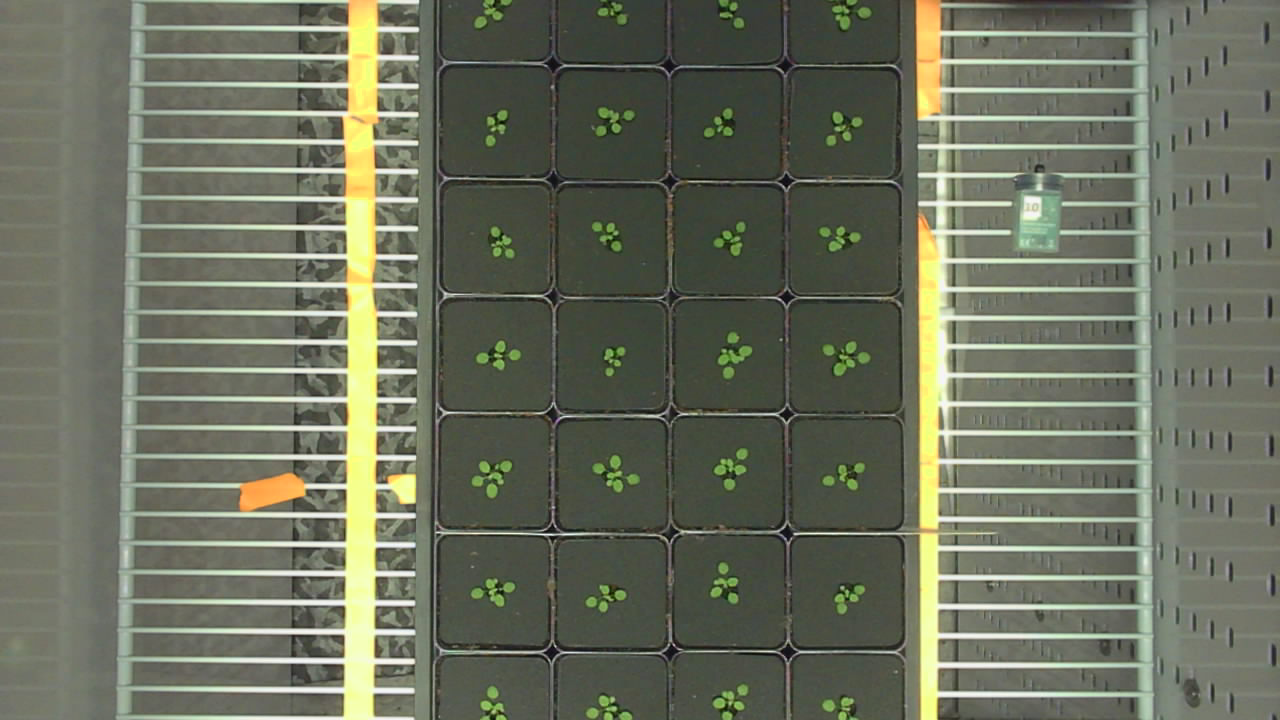
\includegraphics[width=.47\textwidth]{Figures/rawImages/a.png}\\
%Arabidopsis \\
%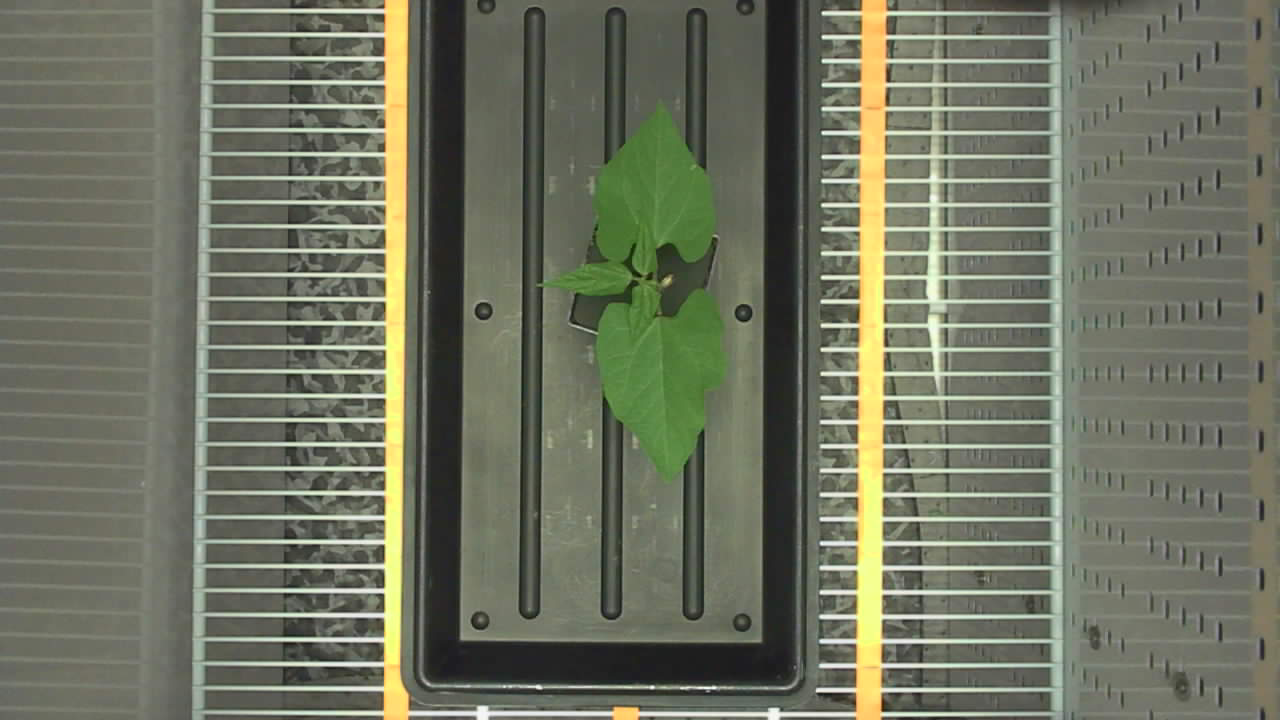
\includegraphics[width=.47\textwidth]{Figures/rawImages/b.png}\\
%   Bean \\
%\end{tabular}
%\caption{RGB color images of Arabidopsis and bean plants. }
%\label{fig:rawIm}
%\end{centering}
%\end{figure}


\begin{table*}[t!]
\begin{center}
\caption{Summary of Arabidopsis and Bean databases.}
\label{tab:stat}
\begin{tabular}{c|c|c|c|c|c}
      \hline
      % after \\: \hline or \cline{col1-col2} \cline{col3-col4} ...
      Plants     & Subjects & Days & Images/Day & Total Images & Annotated Images \\
      \hline
      Arabidopsis &  $16$      &  $9$   &     $16$     &     $2304\times 4$     &       $576\times 4$     \\
      \hline
      Bean        &   $5$      &  $5$   &     $14$     &     $350\times 4$       &       $175\times 4$  \\
      \hline
\end{tabular}
\end{center}
\end{table*}



\begin{table*}
\begin{center}
\caption{Plant image resolution of Arabidopsis and Bean databases.}
\label{tab:resolution}
\begin{tabular}{c|c|c|c|c}
      \hline
      % after \\: \hline or \cline{col1-col2} \cline{col3-col4} ...
      Plants     & Fluorescence       & IR        & RGB      & Depth     \\
      \hline
      Arabidopsis &  $\sim$$240\times240$ &  $\sim$$240\times240$  & $\sim$$120\times120$  & NA  \\
      %\hline
      Bean        & $1000\times640$ & $1000\times640$ & $380\times720$ & $90\times190$    \\
      \hline
\end{tabular}
\end{center}
\end{table*}
